\documentclass[a4paper,12pt]{article}
\usepackage[top = 2.5cm, bottom = 2.5cm, left = 2.5cm, right = 2.5cm]{geometry}
\usepackage[T1]{fontenc}
\usepackage[utf8]{inputenc}
\usepackage{multirow} 
\usepackage{booktabs} 
\usepackage{graphicx}
\usepackage[spanish]{babel}
\usepackage{setspace}
\setlength{\parindent}{0in}
\usepackage{float}
\usepackage{fancyhdr}
\usepackage{amsmath}
\usepackage{amssymb}
\usepackage{amsthm}
\usepackage[numbers]{natbib}
\newcommand\Mycite[1]{%
	\citeauthor{#1}~[\citeyear{#1}]}
\usepackage{graphicx}
\usepackage{subcaption}
\usepackage{booktabs}
\usepackage{etoolbox}
\usepackage{minibox}
\usepackage{hyperref}
\usepackage{xcolor}
\usepackage[normalem]{ulem}
 \useunder{\uline}{\ul}{}
\usepackage[skins]{tcolorbox}
%---------------------------

\newtcolorbox{cajita}[1][]{
	 #1
}

\newenvironment{sol}
{\renewcommand\qedsymbol{$\square$}\begin{proof}[\textbf{Solución.}]}
	{\end{proof}}

\newenvironment{dem}
{\renewcommand\qedsymbol{$\blacksquare$}\begin{proof}[\textbf{Demostración.}]}
	{\end{proof}}

\newtheorem{problema}{Problema}
\newtheorem{definicion}{Definición}
\newtheorem{ejemplo}{Ejemplo}
\newtheorem{teorema}{Teorema}
\newtheorem{corolario}{Corolario}[teorema]
\newtheorem{lema}[teorema]{Lema}
\newtheorem{prop}{Proposición}
\newtheorem*{nota}{\textbf{NOTA}}
\renewcommand\qedsymbol{$\blacksquare$}
\usepackage{svg}
\usepackage{tikz}
\usepackage[framemethod=default]{mdframed}
\global\mdfdefinestyle{exampledefault}{%
linecolor=lightgray,linewidth=1pt,%
leftmargin=1cm,rightmargin=1cm,
}




\newenvironment{noter}[1]{%
\mdfsetup{%
frametitle={\tikz\node[fill=white,rectangle,inner sep=0pt,outer sep=0pt]{#1};},
frametitleaboveskip=-0.5\ht\strutbox,
frametitlealignment=\raggedright
}%
\begin{mdframed}[style=exampledefault]
}{\end{mdframed}}
\newcommand{\linea}{\noindent\rule{\textwidth}{3pt}}
\newcommand{\linita}{\noindent\rule{\textwidth}{1pt}}

\AtBeginEnvironment{align}{\setcounter{equation}{0}}
\pagestyle{fancy}

\fancyhf{}









%----------------------------------------------------------
\lhead{\footnotesize Geometría Moderna}
\rhead{\footnotesize  Rudik Roberto Rompich}
\cfoot{\footnotesize \thepage}


%--------------------------

\begin{document}
 \thispagestyle{empty} 
    \begin{tabular}{p{15.5cm}}
    \begin{tabbing}
    \textbf{Universidad del Valle de Guatemala} \\
    Departamento de Matemática\\
    Licenciatura en Matemática Aplicada\\\\
   \textbf{Estudiante:} Rudik Roberto Rompich\\
   \textbf{Correo:}  \href{mailto:rom19857@uvg.edu.gt}{rom19857@uvg.edu.gt}\\
   \textbf{Carné:} 19857
    \end{tabbing}
    \begin{center}
        MM2031 - Geometría Moderna - Catedrático: María Eugenia Contreras Pinillos\\
        \today
    \end{center}\\
    \hline
    \\
    \end{tabular} 
    \vspace*{0.3cm} 
    \begin{center} 
    {\Large \bf  HT 1
} 
        \vspace{2mm}
    \end{center}
    \vspace{0.4cm}
%--------------------------

\begin{problema}
	Dado un triángulo si en él unimos los puntos medios de los lados del triángulo obtenemos un nuevo triángulo.
	\begin{figure}[H]
		\centering 
		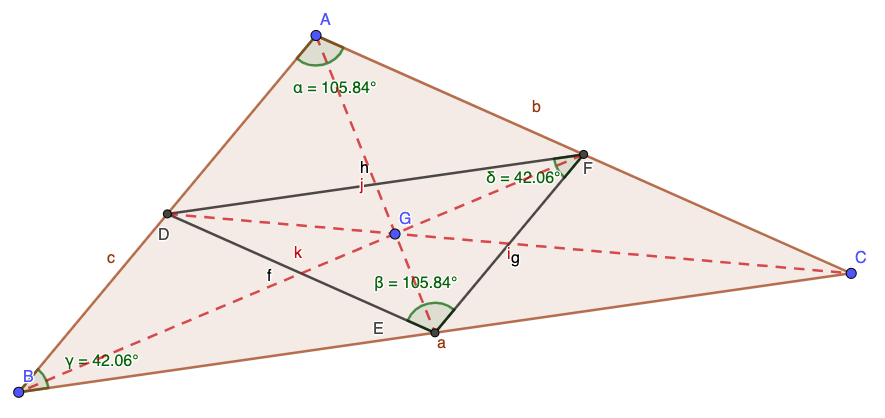
\includegraphics[scale=0.3]{Images/1}
	\end{figure}
	\begin{enumerate}
		\item Demuestre que el nuevo triángulo es homotético al triángulo original. 
		\begin{dem}
			Por el teorema del punto medio, $DF=\frac{1}{2}BC$, $EF=\frac{1}{2}AB$ y $DE=\frac{1}{2}AC$. Por lo tanto, por el criterio SSS para triángulos, comprobamos que $\triangle DEF\cong \triangle ABC$; lo que quiere decir que es homotético. 
		\end{dem}
		\item Obtenga el valor de la constante de homotecia.
		\begin{sol}
			Si usamos la demostración anterior, determinamos que por ejemplo $DF=BE$,  $DE=AF$, $EF=BD$ sucesivamente hasta determinar que se formaron 4 triángulos congruentes. Entonces, de homotecia es $1/4$. 
		\end{sol}
		\item Determine el centro de homotecia.
		\begin{sol}
			Como sabemos que el segundo triángulo es homotético y congruente al original. Además, 
			$$\frac{DE}{AC}=\frac{DF}{BC}=\frac{EF}{AB}$$
			Entonces, se está dividiendo en el punto medio y por lo tanto, podemos concluir que $G$ es el punto medio. 
		\end{sol}
	\end{enumerate}
\end{problema}


\begin{problema}
	 Sea ABCD un cuadrilátero cíclico convexo, cuyas diagonales se cortan en O, entonces
	$$
	|A B||B C||O D|=|C D||D A||B O|
	$$
		\begin{figure}[H]
		\centering 
		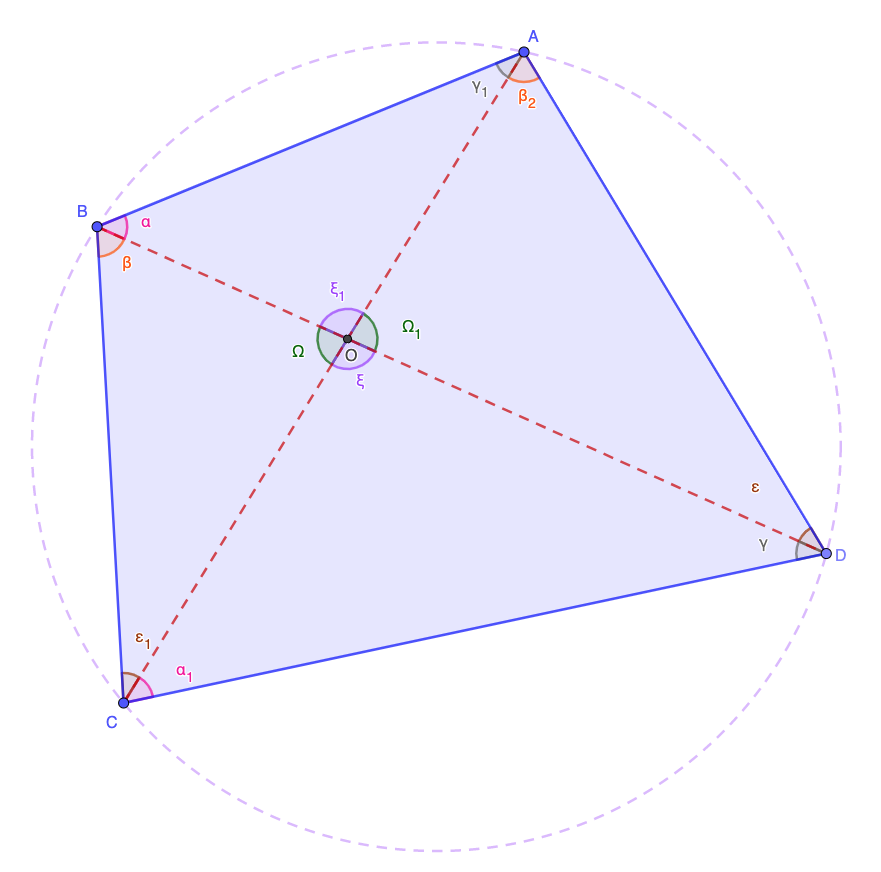
\includegraphics[scale=0.3]{Images/3}
	\end{figure}
	\begin{dem}
		Por la propiedad de ángulos inscritos en un cuadrilátero, sabemos 
		\begin{align*}
			\alpha : & \angle ABD \cong \angle ACD\\
			\beta : & \angle DAC \cong \angle DBC\\
			\gamma : & \angle CAB \cong \angle CDB\\
			\varepsilon : & \angle BCA \cong \angle BDA\\
		\end{align*},
	Además, por la definición de convexidad, 
	\begin{align*}
		\Omega : & \angle AOD \cong \angle COB\\
		\xi : & \angle BOA \cong \angle DOC\\
	\end{align*}
Ahora bien, vamos a utilizar la ley de senos en los siguientes triángulos: 
\begin{align*}
	\triangle OCD: & \frac{OC}{\sen \gamma}=\frac{OD}{\sen \alpha}\implies \frac{OC}{OD}=\frac{\sen \gamma}{\sen \alpha}\\
	\triangle BCO: & \frac{OC}{\sen \beta}=\frac{BO}{\sen \varepsilon}\implies \frac{OC}{BO}=\frac{\sen \beta}{\sen \varepsilon}\\
	\triangle BCD: & \frac{CD}{\sen\beta}=\frac{BC}{\sen \gamma}\implies \frac{CD}{BC}=\frac{\sen \beta }{\sen \gamma}\\
	\triangle BDA: & \frac{AD}{\sen \alpha}=\frac{AB}{\sen\varepsilon}\implies \frac{AD}{AB}=\frac{\sen \alpha}{\sen\varepsilon}\\
\end{align*}
$$\implies \frac{\frac{OC}{OD}}{\frac{OC}{BO}}=\frac{OC\cdot BO}{OD\cdot OC}=\frac{\sen \gamma \cdot \sen \varepsilon}{\sen \alpha \cdot \sen \beta}=\frac{BC}{CD}\cdot \frac{AB}{AD}$$
$$\implies \frac{BO}{OD}=\frac{BC}{CD}\cdot \frac{AB}{AD}$$
Por lo tanto, por el valor absoluto y despejando: 
	$$
|A B||B C||O D|=|C D||D A||B O|
$$
	\end{dem}
\end{problema}

\begin{problema}
	Se tiene un pentágono regular:
		\begin{figure}[H]
		\centering 
		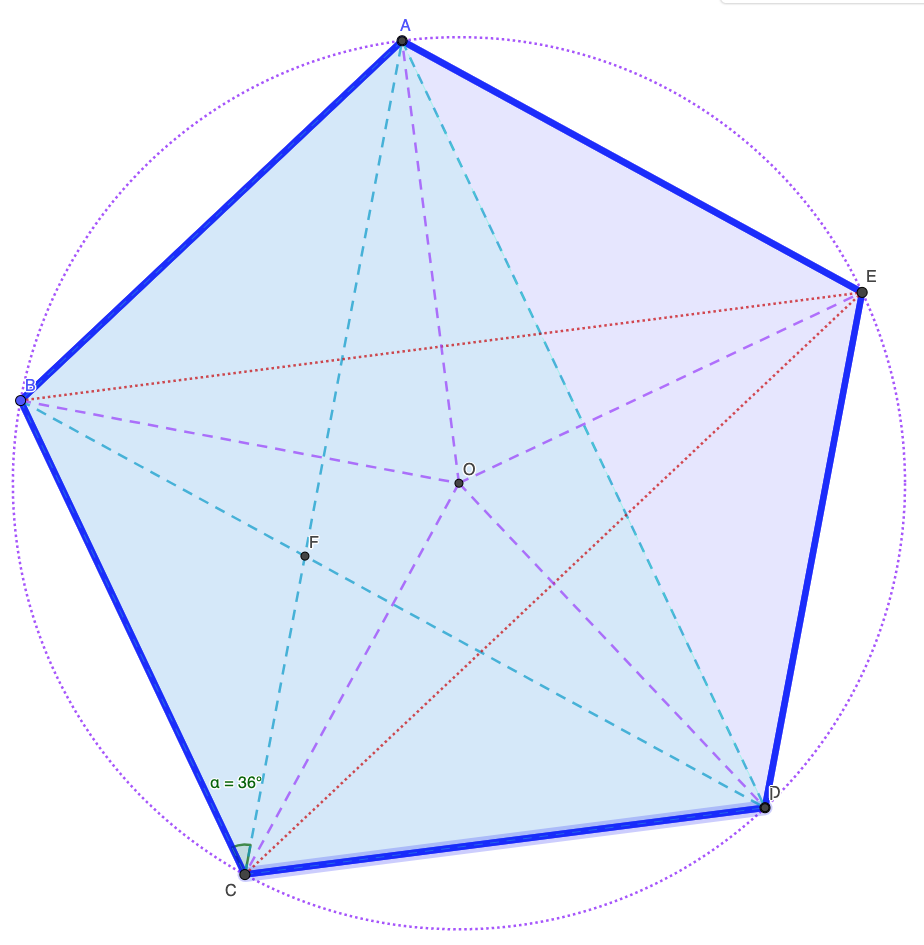
\includegraphics[scale=0.3]{Images/4}
	\end{figure}
	\begin{enumerate}
	   \item Encuentre la razón que existe entre la diagonal $\mathrm{y}$ su lado.
	   	\begin{dem}
	   	Nótese que podemos formar un cuadrilátero inscrito en el circulo del pentágono. $\implies$ Por el teorema de Ptolomeo, 
	   	$$AC\cdot BD = AB\cdot CD+AD\cdot BC$$
	   	$\implies$ Como es una figura regular, sus diagonales miden lo mismo, igualmente sus lados miden lo mismo. Digamos que los lados están representados por $l$ y sus diagonales por $d$, entonces: 
	   	$$d\cdot d = l\cdot l+d\cdot l\implies d^2 = l^2 +d\cdot l$$
	   	La razón está dado por $r=d/l$, entonces dividamos todo por $l^2$: 
	   	$$\implies \frac{d^2}{l^2}=1+ \frac{d}{l}\implies r^2=1+r\implies r^2-r-1=0$$
	   	Usando la fórmula cuadrática: 
	   	$$r=\frac{1\pm\sqrt{5}}{2}$$
	   	Como nos interesa la razón, solo vamos a tomar en cuenta el número positivo.  Por lo tanto, 
	   	$$\frac{d}{l}=\frac{1+\sqrt{5}}{2}$$
	   \end{dem}
	   \item Utilice lo anterior para determinar el $\cos 36^{\circ}$.
	   	\begin{dem}
	   Usando la ley de cosenos dada como, 
	   $$c=\sqrt{a^2+b^2-2ab\cos\gamma}\implies \cos\gamma =\frac{c^2-a^2-b^2}{-2ab}$$
	   Dado $a=1+\sqrt{5}$ y $b=c= 2$, concluimos:
	   $$\implies \cos36^\circ = \frac{(2)^2-(1+\sqrt{5})^2-(2)^2}{-2(1+\sqrt{5})(2)}= \frac{1+\sqrt{5}}{4}$$ 
	   \end{dem}
	   \item Obtenga la razón entre el lado y el radio del circulo que lo suscribe.
	   	\begin{dem}
	   		Por las propiedades de los triángulos regulares, los ángulos que forman los radios en el centro (las líneas moradas en la figura) son de $72^\circ$ y los adyacentes a los lados de $54^\circ$. 
	   		Entonces, por ley de senos: 
	   		$$\frac{2}{\sen72}=\frac{OD}{\sen 54}$$
	   	La razón es: 
	   	$$\frac{1}{2}\sqrt{10-2\sqrt{5}}$$
	   	[según la calculadora :(]
	   \end{dem}
	\end{enumerate}
\end{problema}





%---------------------------
\bibliographystyle{apa}
\bibliography{referencias.bib}

\end{document}